\section{Prototyp}\label{sec:prototypPraktisch}

Bevor die Erstellung von Prototypen für den Nutzungskontext beginnen konnte, müssen einige Überlegungen angestellt werden.
Im Gegensatz zu einigen anderen Kontexten muss hier Software von Grund auf entwickelt werden.
Hierzu wird zunächst überlegt, wie eine auf \autoref{sec:sollSzenario} aufbauende Software beschaffen sein muss.
Im zweiten Schritt werden konkrete designspezifische Überlegungen angestellt. 
Diese werden anhand einiger Mockups vorgestellt.

\subsection{Vorüberlegungen}

Aus dem in \autoref{sec:sollSzenario} zu findenden Soll-Szenario ist abzuleiten, dass die Software über mindestens zwei Hauptansichten verfügen muss.
Dabei eignet sich eine dieser Ansichten (ab hier Übersicht genannt) zur Darstellung der an der Durchsuchung beteiligten Personen und Objekten.
Diese soll vorzugsweise auf einem interaktiven Touch Display (beispielsweise der Firma SmartBoard) betrieben werden, damit alle sich im Raum befindlichen Personen eine möglichst gute Einsicht auf diese Übersicht haben.
Die Übersicht soll neben den Personen und Objekten ebenfalls alle eingegebenen Informationen darstellen.
Dies soll anhand einer Timeline geschehen, welche sich an dem Design einer Twitter Timeline\footnote{\url{https://twitter.com/TwitterSupport/status/1501989523588358145}} orientiert.
Des Weiteren soll diese Ansicht über eine Filter Funktion für Objekte verfügen, welche des den Nutzenden erlaubt, schnell und einfach Zugang zu den gewünschten Informationen zu erhalten.

Bei der zweiten Ansicht handelt es sich um eine Eingabemaske.
Diese wird simultan in mehreren Instanzen auf Notebooks ausgeführt.
Ziel ist es hier, jeder sich im Meldekopf befindlichen Person eine möglichst bequeme Möglichkeit zu geben, zu jeder Zeit neue Informationen zu erfassen.
Um diese Produktivität des Systems zu maximieren, soll die Eingabemaske über einige Hilfen verfügen.
Es soll möglich sein, mit Hilfe einer automatischen Vervollständigung schnell Personen oder Objekte zu referenzieren.
Ebenso sollen oft verwendete Informationen in Form von Templates gespeichert sein, welche auf Wunsch nur mit den betreffenden Personen und Objekten gefüllt werden müssen.
Damit stets eine Übersicht über alle Vorgänge der Durchsuchung herrscht, soll auch hier die bereits erwähnte Timeline für Informationen eingefügt werden.

Im Idealfall wird das neue System also von mehreren Bildschirmen und Eingabegeräten zur selben Zeit betrieben. 
Bei der Erstellung von Mockups soll darauf geachtet werden, welche Eingabegeräte an den zu den Ansichten vorgesehenen Geräten zur Verfügung stehen.

\subsection{Mockups}

Aus dem soeben festgelegten Konzept werden nun Mockups erstellt.
Wird im Gegensatz zu Mockups nicht rein auf die Anordnung von Elementen, sondern auch auf deren Darstellung geachtet.
Die Mockups sind in zwei Kategorien eingeteilt. 
Zuerst zu sehen sind Mockups, welche das Design der Eingabemaske wiedergeben.
Auf diese folgen Mockups zum Übersichtsbildschirm.
Aus Gründen des Umfangs umfasst dieses Dokument nicht alle erstellten Mockups.
Der Inhalt dieser wird jedoch durch textuelle Beschreibungen ersetzt.

\subsubsection{Eingabemaske}

Die Mockups der Eingabemaske spiegeln das Verschieben einer Person zu einem neuen Objekt wider.
\autoref{fig:inputStart} zeigt hierbei den initialen Zustand der Eingabemaske.
Im oberen Bereich finden sich Möglichkeiten Personen und Objekte zu referenzieren, daneben die Funktion zum Laden eines Templates, hier "Vorbereitete Vorgänge" genannt.
In diesem Mockup sind nur zwei Templates zu sehen.
Mehr Templates sollen über die Zeit hinzugefügt werden.
Hierzu muss das Programm des Öfteren Bei Großdurchsuchungen zum Einsatz kommen.
Hierbei werden fehlende Templates schnell ausfindig gemacht.

\begin{figure}[htp]
    \centering
    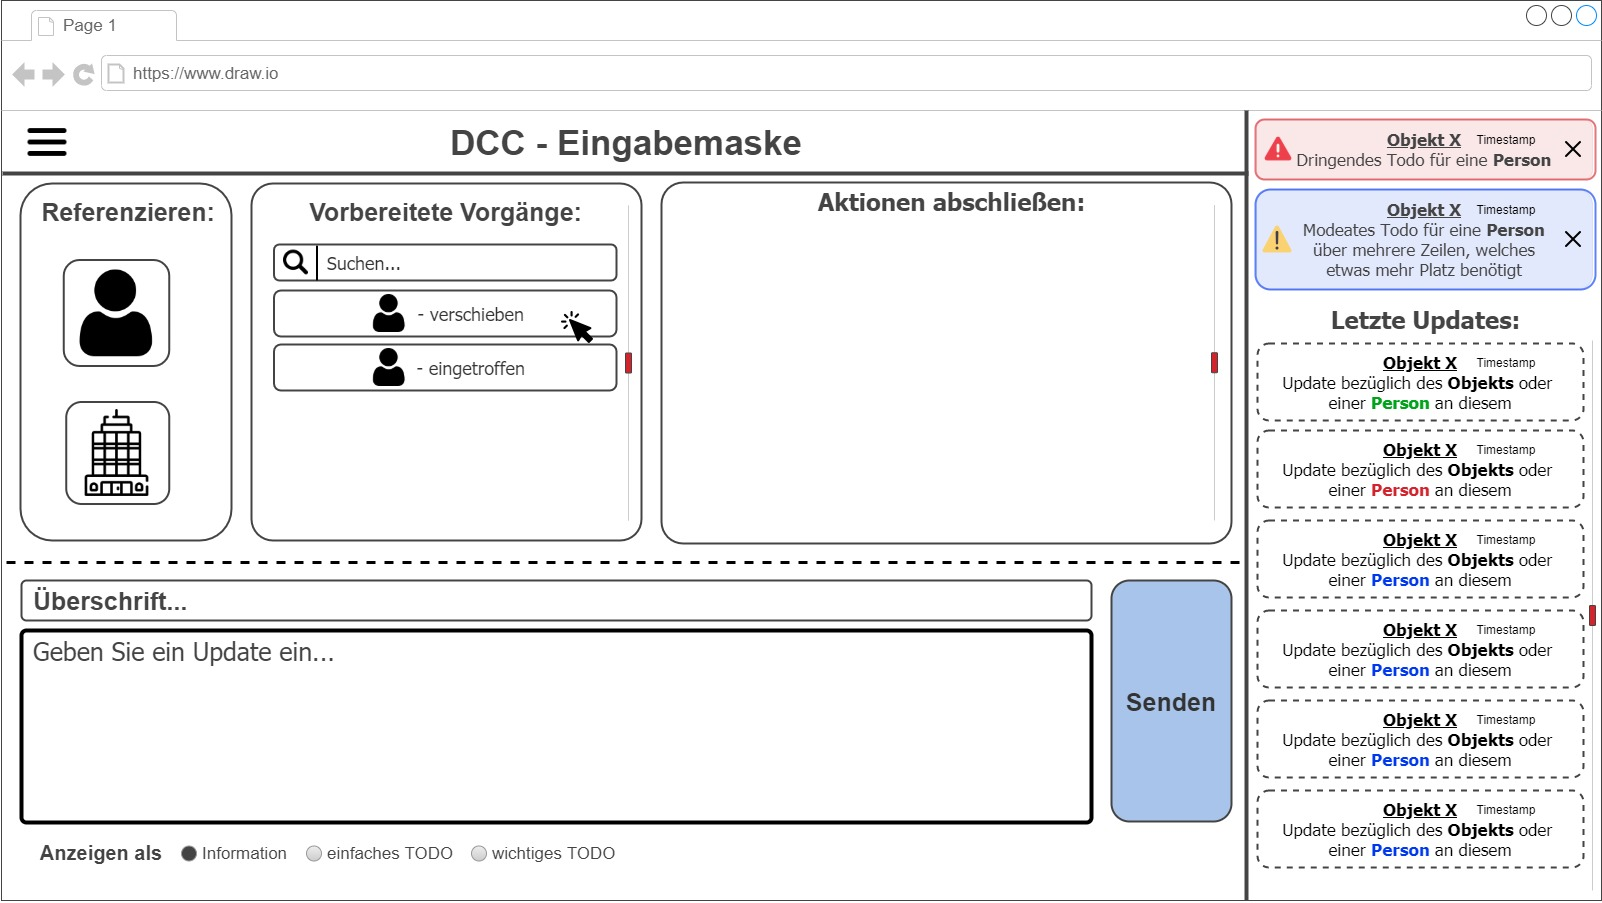
\includegraphics[width=\textwidth]{images/1-MockupsV1/InputScreenStart.jpg}
    \caption{Eingabemaske Start}
    \label{fig:inputStart}
\end{figure}

Rechts neben den Templates findet sich ein Bereich zum Abschließen von Aktionen.
Beispielsweise erscheint dort das bereits ausgefüllte Template "Personen eingetroffen", wenn diese zuvor verschoben wurden.
Unter diesen drei Boxen findet sich die eigentliche Eingabemöglichkeit.
Nutzende geben hier Überschrift und Nachricht ein, bevor sie diese über den Button absenden können.
Unter diesen Eingabefeldern findet sich eine Auswahl für die Darstellung der Updates.
Hier kann zwischen einer normalen Darstellung und zwei angepinnten Varianten entschieden werden.

Diese Wahl wirkt sich direkt auf die rechts dargestellte Timeline aus.
Erkenntlich ist, dass diese über drei Darstellungsarten verfügt.
Weiß steht hier für eine einfache Information, welche keine weiteren Aktionen benötigt.
Blau und Rot stehen für angepinnte Informationen oder auch ToDos. 
Diese werden stets am oberen Ende der Timeline angezeigt.
Über das Kreuz kann ein ToDo als erledigt erklärt werden.
Erledigte ToDos werden in normale Informationen umgewandelt und normal in der Timeline angezeigt.

\begin{figure}[htp]
    \centering
    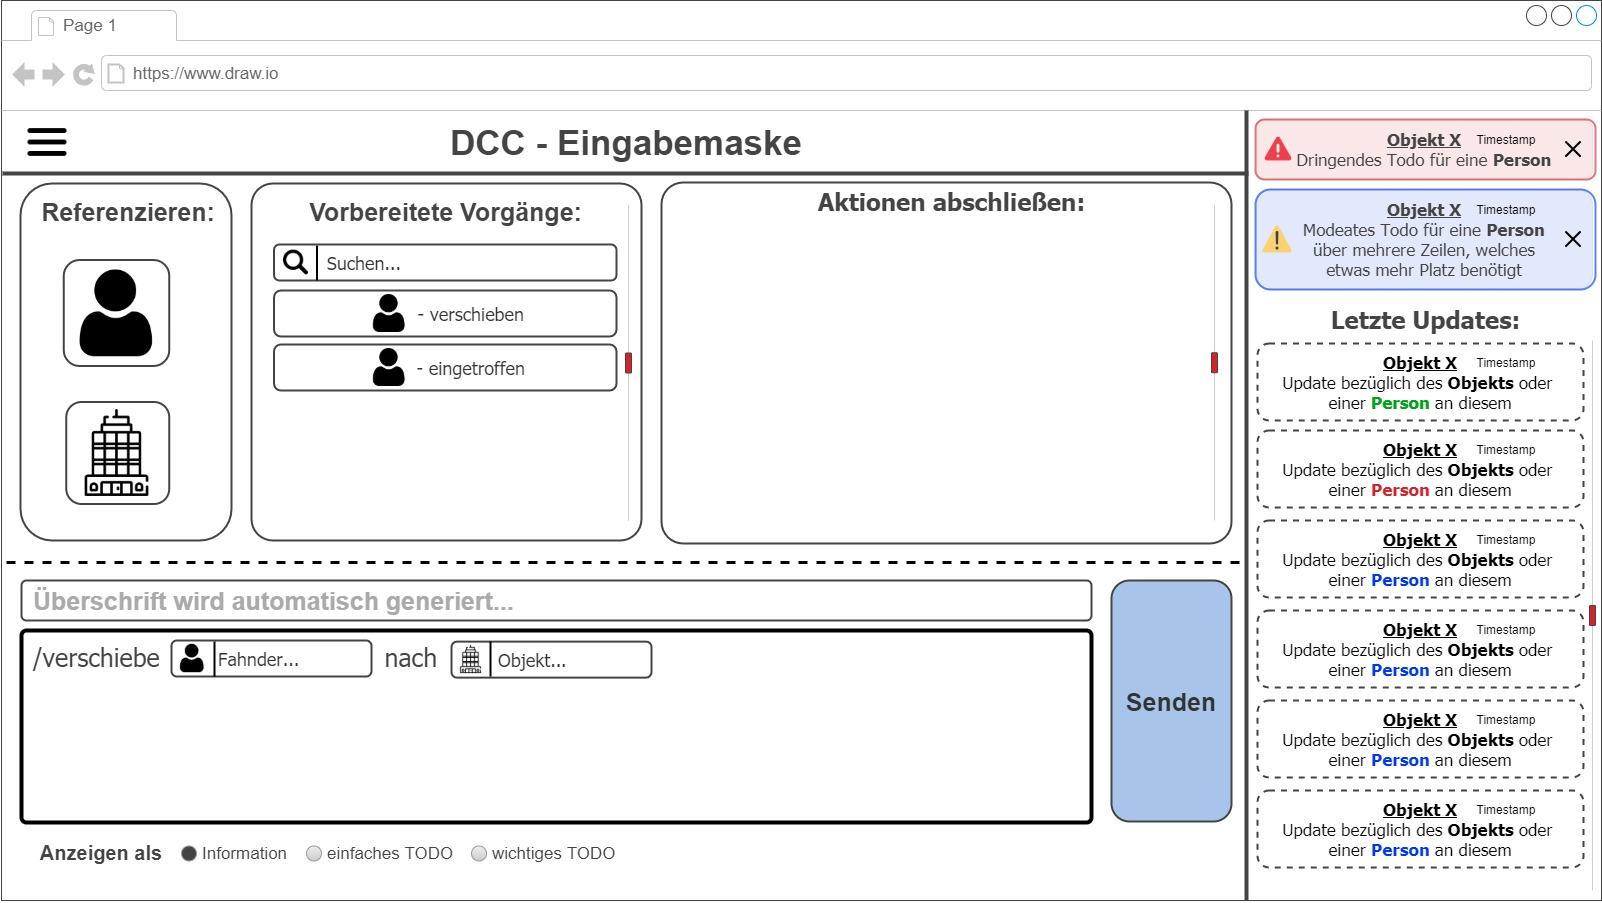
\includegraphics[width=\textwidth]{images/1-MockupsV1/InputScreenMiddle.jpg}
    \caption{Eingabemaske im Vorgang}
    \label{fig:inputMiddle}
\end{figure}

Wie bereits angemerkt stellen diese Mockups den Prozess des Verschiebens einer Person nach.
Hierzu wird nun im in \autoref{fig:inputStart} zu sehenden Mockup auf die Schaltfläche "Person verschieben" geklickt.
Wie erwartet lädt das Programm sodann das ausgewählte Template in die Eingabe.
Das Resultat dessen ist in \autoref{fig:inputMiddle} zu erkennen.

Das Eingabefeld der Überschrift ist nun deaktiviert, da im Fall der Verschiebung von Personen eine automatisch generierte Überschrift verwendet werden soll.
Darunter ist das Template "Person verschieben" zu sehen.
Das dem Text vorangestellt Slash Zeichen indiziert hierbei dem System, dass es sich über eine normale Nachricht hinaus um einen Befehl zum Ändern des Datenmodells handelt.
Neben des Slash Zeichens wurde ein von den Nutzenden auszufüllender Lückentext generiert.
Dieser enthält einen Satz, welcher den ausgewählten Vorgang beschreibt, in diesem Fall "Verschiebe [Person] nach [Objekt]".
Die Lücken können hierbei ausgefüllt werden, indem mit der Maus in sie geklickt wird.

Sollen mehrere Personen verschoben werden, so können mehr Personenfelder generiert werden, indem entweder unter "Referenzieren" auf die Person geklickt wird oder das Zeichen "@" eingefügt wird.
Nach dem Abschicken erkennt das Programm, dass mehrere Personen verschoben wurden und führt die Änderung im Datenmodell dementsprechend aus.

Wurde nun in das Eingabefeld für eine Person geklickt, so öffnet sich ein wie in \autoref{fig:inputEnd} dargestelltes Auswahlfenster, welches die verfügbaren Personen in alphabetischer Reihenfolge anzeigt.
Wird eine Eingabe im Feld getätigt, so passt sich das Auswahlfenster insofern an, dass nur zur aktuellen Eingabe passende Personen angezeigt werden.
Eine Person kann ausgewählt werden, indem mit der Maus auf sie geklickt wird.
Ebenso wird die oberste Person beim Drücken der Tabulator Taste ausgewählt.


\begin{figure}[htp]
    \centering
    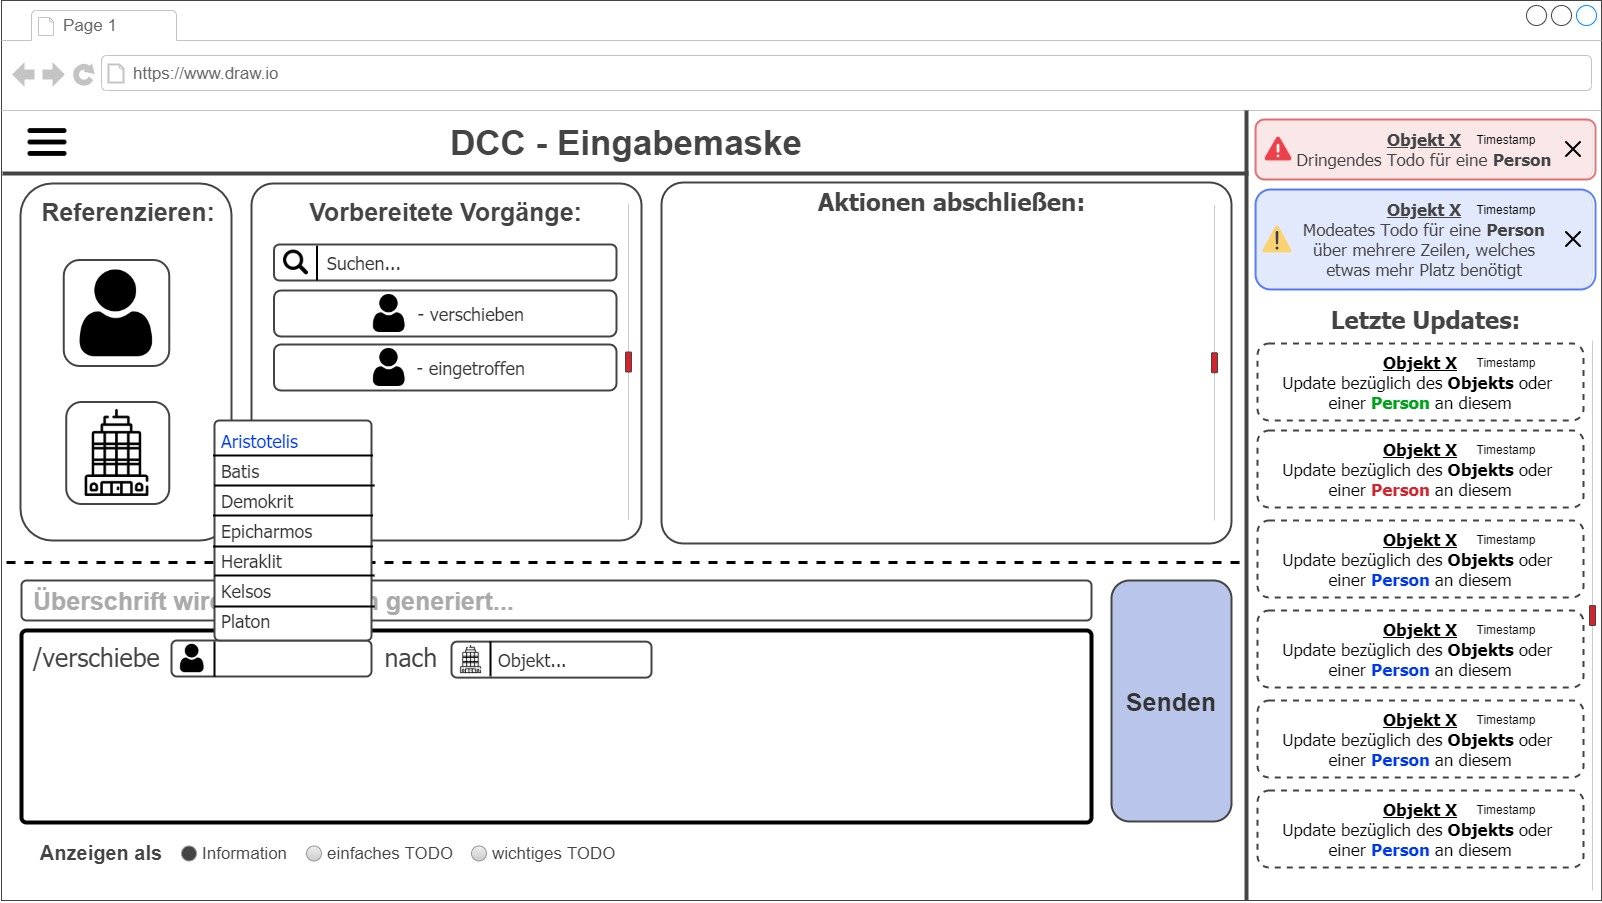
\includegraphics[width=\textwidth]{images/1-MockupsV1/InputScreenEnd.jpg}
    \caption{Eingabemaske Ende}
    \label{fig:inputEnd}
\end{figure}

Ist das Template vollständig ausgefüllt, kann es über die "Senden" Taste abgeschickt werden.
Dabei findet zunächst eine Konsistenzprüfung der angegebenen Daten statt.
Werden Fehler im Ausfüllprozess erkannt, so wird das Template nicht abgeschickt und den Nutzenden eine Fehlermeldung angezeigt.

Nach dem Abschicken des Templates werden die Eingabefelder geleert, sowie die Eingabe einer Überschrift wieder aktiviert.
In der Timeline erscheint ein neues Item, welches Titel und Inhalt des soeben abgeschickten Templates trägt.
Das Slash Zeichen wird dabei entfernt und Personen und Objektfelder durch Namen und Objektkennungen ersetzt.

Damit ist der Prozess des Verschiebens in der Eingabemaske abgeschlossen.
Es folgt eine Darstellung desselben Prozesses auf dem Übersichtsbildschirm.

\newpage
\subsubsection{Übersichtsbildschirm}

Nach abgeschlossenem Studieren des Konzepts der Eingabemaske wird nun ein Fokus auf den Übersichtsbildschirm gelegt.
\autoref{fig:viewStart} zeigt diesen vor der Durchführung des Verschiebens von Personen.
Dabei ist der linke Teil des Bildschirms der Kern des Übersichtsbildschirm.
Dieser besteht aus einem Bereich, welcher die Filterung der angezeigten Objekte umfasst, den Objekten selbst und einer Zeile, welche Personen anzeigt, welche sich an keinem Objekt befinden.

Seien zunächst die Funktionen des Filters aufgeführt.
Verschiedene Filter können über ein Dropdown Menü gewählt werden.
Dabei werden gewählte Filter rechts neben diesem Menü angezeigt.
Soll ein Filter abgewählt werden, so kann auf das Kreuz neben diesem Filter geklickt werden.
Es stehen einige voreingestellt Filter zur Verfügung.
Dabei handelt es sich beispielsweise um eine Auswahl des Objekttyps (Wohnung, Betrieb, ...) oder das Bundesland, in welchem sich das Objekt befindet.
Zusätzlich können Nutzende eigene Filter erstellen.
Dies funktioniert über ein System von Tags.
Jedem Objekt können beliebig viele Tags hinzugefügt werden, welche später als Filter gewählt werden können.

\begin{figure}[htp]
    \centering
    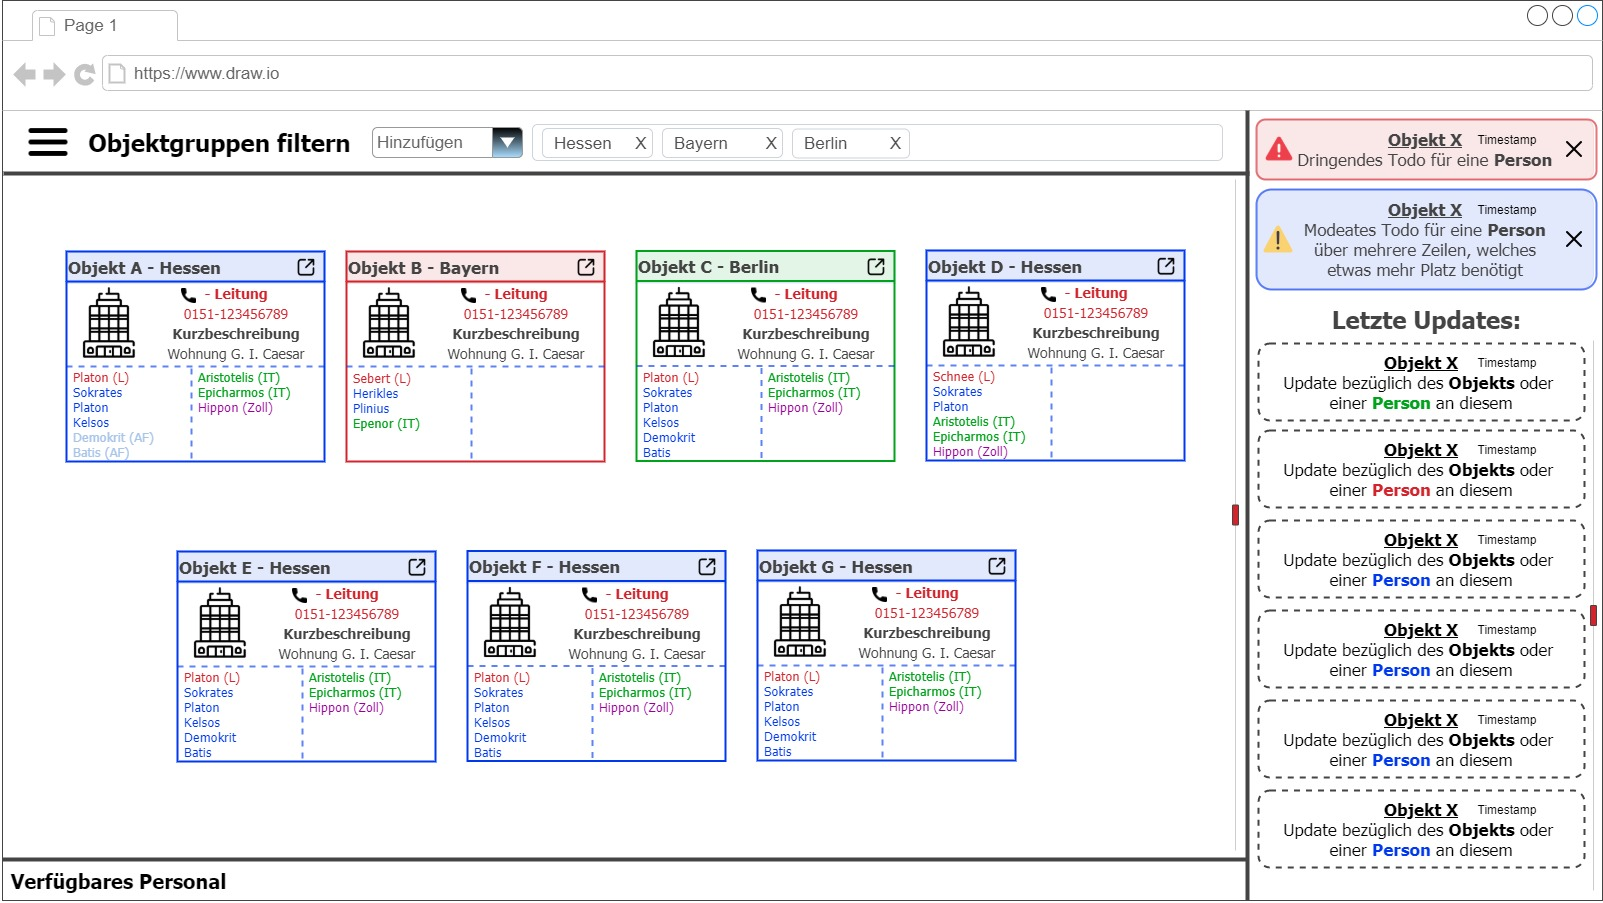
\includegraphics[width=\textwidth]{images/1-MockupsV1/ViewScreenLessBeforeMove.jpg}
    \caption{Übersichtsbildschirm Start}
    \label{fig:viewStart}
\end{figure}

Objekte werden als farbige Kästen dargestellt.
Dabei indiziert die Farbe das Bundesland des Objekts.
Zu jedem Objekt sind Kennung, Bundesland, Telefonnummer der Objektleitung, eine Kurzbeschreibung und das dort tätige Personal direkt ersichtlich.
Weitere Informationen zu einem Objekt können über den Button oben rechts angezeigt werden.
Dies wird durch ein Modalfenster realisiert.
Ebenso in der Überlegung befand sich hier ein an den Home-Bildschirm von Smartphones angelegtes System aus mehreren Ansichten, welche durch wischen geändert werden können.
Zu Gunsten des Überblicks fiel die Wahl jedoch auf das Modalfenster.
Personen sind ebenfalls eingefärbt.
Sie sind somit nach ihrem Einsatzgebiet gruppiert.

Unter den Objekten werden alle momentan verfügbaren Personen angezeigt.
Eine Person gilt als verfügbar, sobald sie keinem Objekt zugeordnet ist.
Neben einer Person wird hier ebenfalls ihr letzter Aufenthaltsort angezeigt.

\begin{figure}[htp]
    \centering
    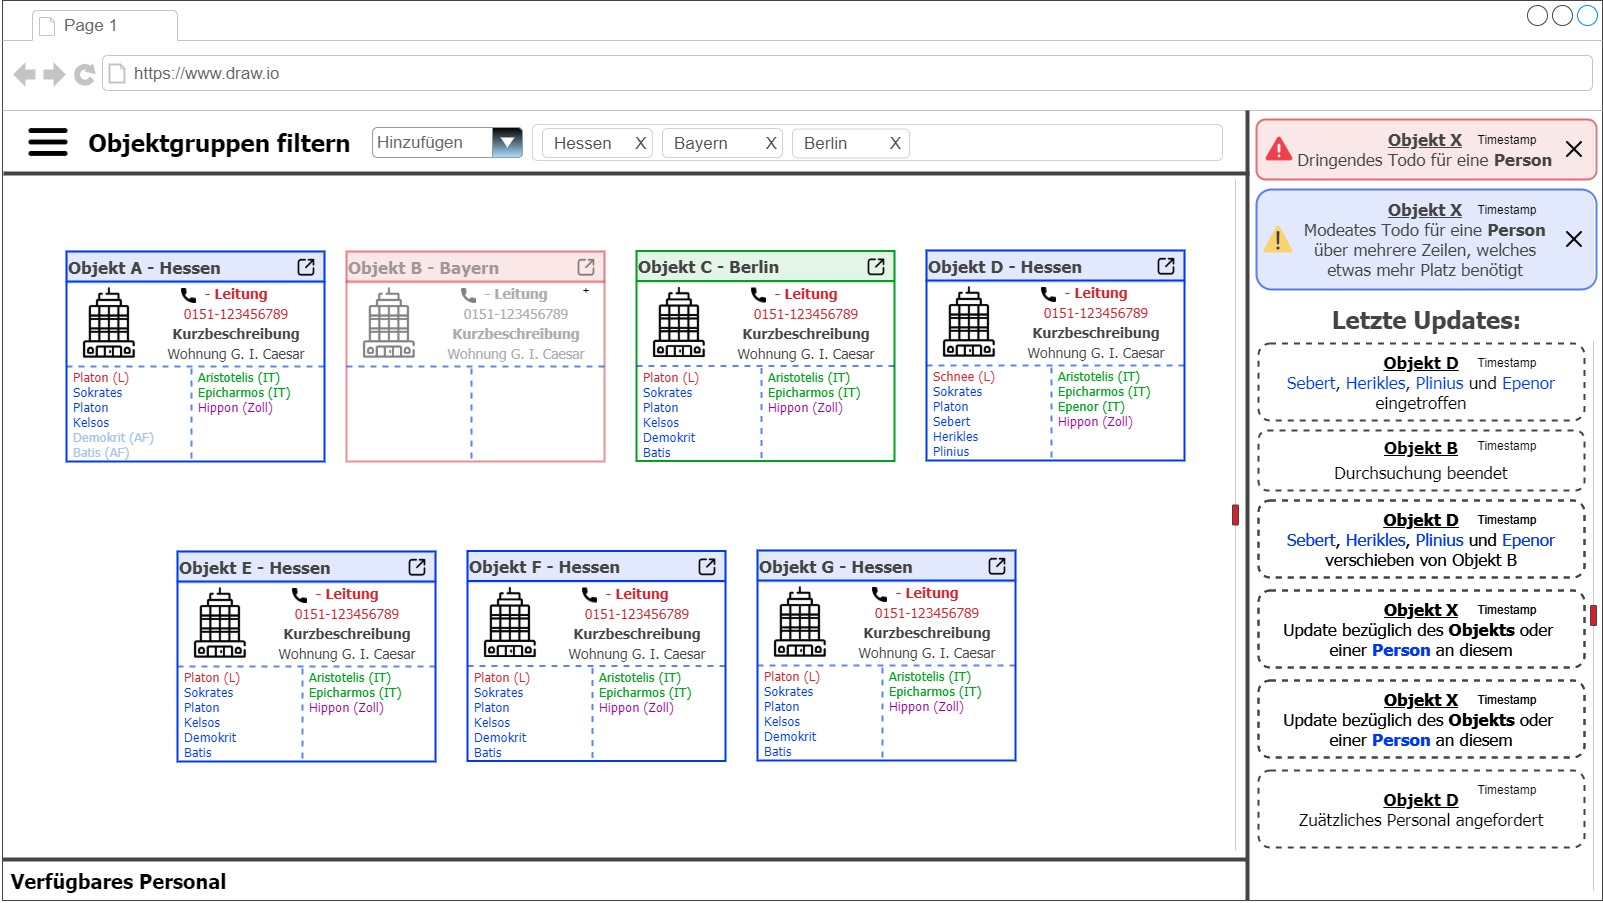
\includegraphics[width=\textwidth]{images/1-MockupsV1/ViewScreenLessAfterMove.jpg}
    \caption{Übersichtsbildschirm Ende}
    \label{fig:viewEnd}
\end{figure}

Es werden nun alle Personen von Objekt B nach Objekt D verschoben.
Darüber hinaus wird die Durchsuchung in Objekt B als abgeschlossen markiert.
In \autoref{fig:viewEnd} ist nun ein Mockup zu sehen, welches diesen Stand abbildet.
Um anzuzeigen, dass eine Durchsuchung abgeschlossen ist, wird das betroffene Objekt ausgegraut dargestellt.
Die dort tätigen Personen sind nun unter Objekt D zu finden.
Ebenso ist in der Timeline die Information zur Aktion zu sehen.

Die Darstellung von sich momentan auf der Anfahrt zu einem Objekt befindlichen Personen ist ebenfalls \autoref{fig:viewEnd} zu entnehmen.
Hier befinden sich die Personen Demokrit und Batis in Anfahrt auf Objekt A. 
Diese werden leicht blass dargestellt.
Ebenso ist ihren Namen ein (AF) als Abkürzung für "Anfahrt" angehangen.

Diese Konzepte wurden ebenso in Form eines gecodeten Prototyps umgesetzt. 
Bei diesem wurde jedoch zunächst auf Funktionalität und weniger auf Aussehen geachtet.
Somit wurde sich entschlossen, im Rahmen dieser Arbeit nur die Mockups zu zeigen.
Beide Prototypen werden im nächsten Schritt der Kontextperson präsentiert.